\chapter{Введение в предметную область} \label{ch2}

В начале XXI века человечество вступило в эпоху информации,
характеризующуюся беспрецедентным ростом объемов генерируемых и накапливаемых данных.
Этот феномен, получивший название "Большие данные" (Big Data), стал одной из определяющих тенденций технологического и социально-экономического развития.
Большие данные описываются не просто их колоссальным объемом (Volume), измеряемым в петабайтах и экзабайтах, но и другими ключевыми характеристиками.
К ним относятся высокая скорость (Velocity) поступления и необходимость быстрой обработки, часто в режиме реального времени,
а также чрезвычайное разнообразие (Variety) форматов – от структурированных данных в реляционных таблицах до неструктурированных текстов,
изображений, видео, аудиопотоков, данных с сенсоров и логов веб-серверов.
Нередко выделяют и дополнительные характеристики, такие как достоверность (Veracity),
указывающая на неопределенность и возможное наличие шумов, неточностей или пропусков в данных, и ценность (Value), подчеркивающая потенциальную пользу, которую можно извлечь из анализа этих данных [11].

Движущими силами этого информационного взрыва стали повсеместная цифровизация бизнес-процессов, распространение интернета и мобильных устройств, рост популярности социальных сетей, развитие технологий Интернета вещей (IoT), когда миллиарды устройств непрерывно генерируют данные об окружающей среде и своем состоянии. Традиционные подходы к хранению и обработке данных, основанные на реляционных базах данных и централизованных вычислениях, оказались неспособны эффективно справляться с такими масштабами, скоростью и разнообразием информации [12].

Понимание того, что эти огромные массивы данных содержат скрытые закономерности, тенденции и знания, привело к формированию новой парадигмы. Вместо того чтобы рассматривать данные лишь как побочный продукт деятельности, организации начали видеть в них стратегический актив. Способность собирать, обрабатывать, анализировать большие данные и извлекать из них ценную информацию (insights) превратилась в критически важное конкурентное преимущество.
Применение анализа больших данных охватывает практически все сферы деятельности:
\begin{itemize}
	\item Бизнес и ритейл: Персонализация маркетинговых предложений, оптимизация цепочек поставок, прогнозирование спроса, анализ потребительского поведения, управление рисками, обнаружение мошенничества [13].
	\item Наука: Ускорение исследований в геномике, астрономии, физике частиц[14], климатологии, материаловедении.
	\item Здравоохранение: Персонализированная медицина, анализ медицинских изображений, прогнозирование эпидемий, оптимизация работы клиник, разработка новых лекарств.
	\item Производство: Предиктивное обслуживание оборудования, контроль качества продукции, оптимизация производственных процессов.
	\item Государственное управление: Улучшение городских служб ("умный город"), анализ транспортных потоков, прогнозирование и предотвращение чрезвычайных ситуаций, повышение эффективности государственных услуг.
	\item Финансы: Алгоритмический трейдинг, оценка кредитоспособности, выявление финансовых махинаций.
\end{itemize}
Таким образом, большие данные – это не просто технологический вызов, связанный с хранением и обработкой информации. Это фундаментальный сдвиг, открывающий новые возможности для инноваций, повышения эффективности и создания ценности во всех аспектах человеческой деятельности. Умение работать с большими данными становится необходимым навыком для специалистов различных профилей, а построение надежной и эффективной инфраструктуры для их обработки – ключевой задачей для организаций, стремящихся сохранить и укрепить свои позиции в современном мире [15]. Неспособность адаптироваться к этой новой реальности и использовать потенциал больших данных может привести к потере конкурентоспособности и отставанию в развитии.
\section{Программные системы для работы с большими данными} \label{ch2:system_description}
Рассмотрим ключевые компоненты нашей платформы данных: от источников до BI-уровня, указав, для чего каждый инструмент служит, какие задачи решает и какую роль играет в общей системе. Инструменты выбраны исходя из доклада Smart Data 2024 - State of Data RU Edition[10].
% TODO: разделить на обобщенные слова: хранилище данных, брокер сообщений и тд
\begin{enumerate}[1.]
	\item СУБД PostgreSQL
	      PostgreSQL выступает в платформе в роли традиционного реляционного источника данных[16]. Он хранит структурированную информацию и обеспечивает гарантии ACID[17], сложные SQL-запросы и транзакционные операции. В рамках нашей архитектуры PostgreSQL отвечает за сохранность «исторических» и «оперативных» данных, а также выступает отправной точкой для потоковой репликации Change Data Capture[18] при помощи Debezium[19]. Основная цель PostgreSQL – быть надежным первоисточником, от которого запускаются процессы инкрементального экспорта изменений и пакетной выгрузки данных.
	\item S3-хранилище (Minio)
	      Minio в нашей платформе реализует объектное хранилище, совместимое с API Amazon S3[20]. Оно удобно для размещения файловых загрузок, дампов баз данных, бэкапов, а также — в качестве «озеро данных»[21] — для хранения сырых или уже подготовленных дата-сететов в формате Parquet, CSV, JSON и т. д. Minio обеспечивает горизонтальное масштабирование и возможность распределенного хранения больших объемов неструктурированных данных. Его задача – служить долговременным и недорогим репозиторием для «сырых» данных и результатов пакетных обработок.
	\item Apache Kafka
	      Kafka выступает в роли распределенного брокера сообщений и обеспечивает надежную передачу сообщений между компонентами системы[22]. Она поддерживает высокую пропускную способность, устойчивость к сбоям и возможность горизонтального масштабирования. В платформе Kafka используется для организации событийного потока изменений из PostgreSQL (через Debezium) и передачи данных в потребителей – как для потоковой обработки, так и для загрузки в аналитическое хранилище. Kafka гарантирует упорядоченную доставку, сохранение истории сообщений (ретеншн) и управление потребительскими группами.
	\item Веб-интерфейс для работы с Kafka - AKHQ
	      AKHQ (ранее «Kafka HQ»)[23] – это веб-интерфейс для администрирования и мониторинга кластера Kafka. Он предоставляет удобный UI для просмотра топиков, чтения и отправки сообщений, управления партициями и оффсетами, мониторинга состояния брокеров и групп потребителей. В платформе AKHQ решает задачу оперативного контроля за событиями в шине: инженер может быстро проверить, какие данные передаются, обнаружить «залипания» потребителей или переполненные топики, а также проводить ручную отладку потоков без необходимости работы с CLI или написания собственных скриптов.
	      Debezium и Kafka Connect
	      Debezium – это платформа Change Data Capture (CDC), реализованная в виде набора коннекторов для Kafka Connect[24]. Kafka Connect, в свою очередь, представляет собой фреймворк для потоковой интеграции: он запускает коннекторы-источники (Source Connectors), которые читают данные из внешних систем (PostgreSQL, MongoDB и пр.), преобразуют их в события и записывают в топики Kafka, а также коннекторы-синкеры (Sink Connectors) для доставки данных из Kafka в хранилища (ClickHouse, S3 и т. д.). В нашей архитектуре Debezium Source Connector подключается к WAL PostgreSQL, транслирует изменения в Kafka, а далее отдельный Sink Connector записывает события в ClickHouse или выполняет другие действия. Цель этого двойного инструмента – обеспечить автоматическую и непрерывную синхронизацию данных между компонентами без написания собственного кода обработки.
	\item ClickHouse
	      ClickHouse[25] – это колоночная аналитическая СУБД с высокой скоростью выполнения сложных OLAP-запросов[26] на больших объемах данных. Она оптимизирована для чтения, эффективно сжимает колоночные данные и поддерживает параллельную обработку. В платформе ClickHouse служит основным аналитическим хранилищем, в которое из Kafka через Kafka Connect поступают агрегированные или сырые события. Благодаря своей архитектуре ClickHouse позволяет быстро строить отчеты, дашборды и выполнять ad-hoc анализ, обрабатывая десятки и сотни миллионов строк за доли секунды.
	\item Apache Superset
	      Superset[27] – это BI-платформа с веб-интерфейсом, позволяющая создавать интерактивные дашборды, визуализации и аналитические отчеты поверх различных источников данных (SQL-базы, колоночные хранилища, дата-видео и т. д.). В нашей системе Superset подключается к ClickHouse и предоставляет бизнес-пользователям и аналитикам средства для построения графиков, таблиц, гео-карт и скриптов на SQL. Его цель – закрыть уровень представления данных: от сложных SQL-запросов непосредственного взаимодействия до простого drag-and-drop интерфейса для быстрого получения инсайтов.
\end{enumerate}


В совокупности эти инструменты образуют сквозной конвейер данных: от первичного сбора и хранения, через трансформации и передачу событий, до хранения в аналитической СУБД и визуализации для конечных пользователей. Такое разделение ответственности позволяет использовать лучшие свойства каждого компонента и легко масштабировать или заменять отдельные части платформы по мере роста требований и объемов данных.
Именно поэтому в рамках настоящей работы рассматривается вопрос создания инструмента, призванного облегчить рутинную работу инженера данных по настройке многочисленных компонентов, а также предоставить ему удобное средство для декларативного описания и развертывания конфигураций платформ данных.
Исходя из всего вышеперечисленного, Use-Case диаграмма (диаграмма вариантов использования) разработанного инструмента dpd выглядит следующим образом (\firef{fig:diagram_usecase})
% TODO: сделать диаграмму другой 
\begin{figure}[ht]
	\center
	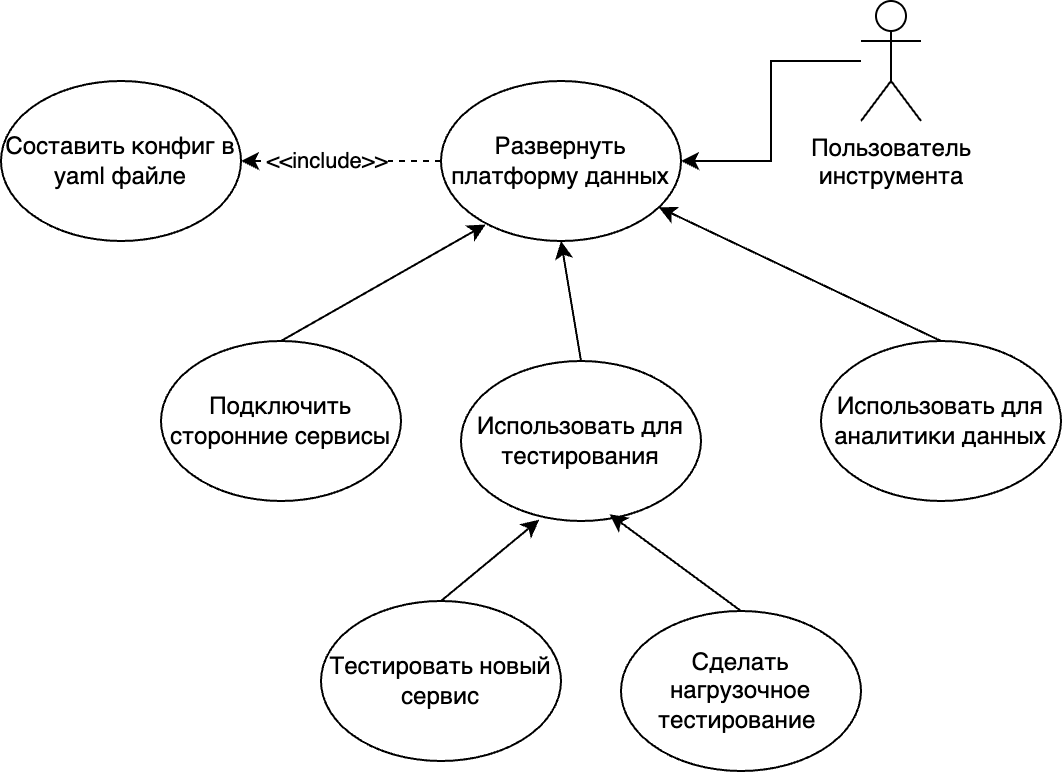
\includegraphics [scale=0.4] {my_folder/images/diagram_usecase}
	\caption{Use-Case диаграмма}
	\label{fig:diagram_usecase}
\end{figure}

% не рекомендуется использовать отдельную section <<введение>> после лета 2020 года
%\section{Введение} \label{ch2:intro}

% Глава посвящена более подробным примерам оформления текстово-графических объектов.

% В параграфе \ref{ch2:title-abbr} приведены примеры оформления многострочной формулы и одиночного рисунка. Параграф \ref{ch2:sec-abbr} раскрывает правила оформления перечислений и псевдокода. В параграфе \ref{ch2:sec-very-short-title} приведены примеры оформления сложносоставных рисунков, длинных таблиц, а также теоремоподобных окружений.


% \section{Название параграфа} \label{ch2:title-abbr} %название по-русски



% %%%%
% %%		
% %%  \input{...} commands are used only to sychronize some parts of the text with the author guide. Authors are free to type the text directly in .tex-files   
% %%  \input{...} комманды используются только, чтобы синхронизировать части текта с рекомендациями авторам. Авторы  вольны вносить текст непосредственно в файл главы  
% %%  
%  \input{my_folder/tex/eq-Galois} % пример двух выравнивания двух формул в окружении align


% На \firef{fig:spbpu-new-bld-autumn-ch2} приведёна фотография Нового научно-исследовательского корпуса СПбПУ.

% 	\begin{figure}[ht] 
% 	\center
% 	\includegraphics [scale=0.27] {my_folder/images/spbpu_new_bld_autumn}
% 	\caption{Новый научно-исследовательский корпус СПбПУ \cite{spbpu-gallery}} 
% 	\label{fig:spbpu-new-bld-autumn-ch2}  
% 	\end{figure}




% \section{Название параграфа} \label{ch2:sec-abbr} %название по-русски

% Название параграфа оформляется с помощью команды \verb|\section{...}|, название главы --- \verb|\chapter{...}|. 


% \subsection{Название подпараграфа} \label{ch2:subsec-title-abbr} %название по-русски


% Название подпараграфа оформляется с помощью команды  \texttt{\textbackslash{}subsection\{...\}}.


% %\subsubsection{Название подподпараграфа} \label{ch2:subsubsec-title-abbr} %название по-русски

% Использование подподпараграфов в основной части крайне не рекомендуется. В случае использования, необходимо вынести данный номер в содержание.	
% Название подпараграфа оформляется с помощью команды  \texttt{\textbackslash{}subsubsecti\-on\{...\}}.



% \input{my_folder/tex/enumeration} % правила использования перечислений	


% Оформление псевдокода необходимо осуществлять с помощью пакета \verb|algorithm2e| в окружении \verb|algorithm|. Данное окружение интерпретируется в шаблоне как рисунок. Пример оформления псевдокода алгоритма приведён на \firef{alg:AlgoFDSCALING}. 


% \input{my_folder/tex/pseudocode-agl-DTestsFDScaling} % пример оформления псевдокода алгоритма 	


% \section{Название параграфа} \label{ch2:sec-very-short-title} %название по-русски



% \input{my_folder/tex/eq-equation-multilined} % пример оформления одиночной формулы в несколько строк

% \input{my_folder/tex/fig-spbpu-sc-four-in-one} % пример подключения 4х иллюстраций в одном рисунке

% %\input{my_folder/tex/fig-spbpu-whitehall-three-in-one} % пример подключения 3х иллюстрации в одном рисунке
% %
% %\input{my_folder/tex/fig-spbpu-main-bld-two-in-one} % пример подключения 2х иллюстраций в одном рисунке

% \input{my_folder/tex/tab-more-than-one-page} % пример подключения таблицы на несколько страциц


% \begin{table} [htbp]% Пример оформления таблицы
% 	\centering\small
% 	\caption{Пример представления данных для сквозного примера по ВКР \cite{Peskov2004}}%
% 	\label{tab:ToyCompare}		
% 		\begin{tabular}{|l|l|l|l|l|l|}
% 			\hline
% 			$G$&$m_1$&$m_2$&$m_3$&$m_4$&$K$\\
% 			\hline
% 			$g_1$&0&1&1&0&1\\ \hline
% 			$g_2$&1&2&0&1&1\\ \hline
% 			$g_3$&0&1&0&1&1\\ \hline
% 			$g_4$&1&2&1&0&2\\ \hline
% 			$g_5$&1&1&0&1&2\\ \hline
% 			$g_6$&1&1&1&2&2\\ \hline		
% 		\end{tabular}
% %	\caption*{\raggedright\hspace*{2.5em} Составлено (или/и рассчитано) по \cite{Peskov2004}} %Если проведена авторская обработка или расчеты по какому-либо источнику	
% 	\normalsize% возвращаем шрифт к нормальному
% \end{table}



% %% please, before using, read the author guide carefully

% \input{my_folder/tex/tab-toy-context-minipage} % пример подключения minipage

% \input{my_folder/tex/fig-spbpu-new-bld-autumn-minipage} % пример подключения minipage




% \input{my_folder/tex/rules-theorem-like-expressions} 

% По аналогии с нумерацией формул, рисунков и таблиц нумеруются и иные текстово-графические объекты, то есть включаем в нумерацию номер главы, например: теорема 3.1. для первой теоремы третьей главы монографии. Команды \LaTeX{} выставляют нумерацию и форматирование автоматически. Полный перечень команд для подготовки текстово-графических и иных объектов находится в подробных методических рекомендациях \cite{spbpu-bci-template-author-guide}. 


% \input{my_folder/tex/rules-list-of-environments} % список некоторых окружений


% \input{my_folder/tex/theorem-example} %пример оформления теоремы


% \input{my_folder/tex/definition-example} %пример оформления определения


% Вместо теоремо-подобных окружений для вставки небольших текстово-графических объектов иногда используются команды. Типичным примером такого подхода является команда \verb|\footnote{text}|\footnote{Внимание! Команда вставляется непосредственно после слова, куда вставляется сноска (без пробела). Лишние пробелы также не указываются внутри команды перед и после фигурных скобок.}, где в аргументе \verb|text| указывают текст \textit{подстрочной ссылки (сноски)}.В них \textit{нельзя добавлять веб-ссылки или цитировать литературу}. Для этих целей используется список литературы. Нумерация сносок сквозная по ВКР без точки на конце выставляется в шаблоне автоматически, однако в каждом приложении к ВКР нумерация, зависящая от номера приложения, выставляется префикс <<П>>, например <<П1.1>> --- первая сноска первого приложения. 




% %\FloatBarrier % заставить рисунки и другие подвижные (float) элементы остановиться


% \section{Выводы} \label{ch2:conclusion}

% Текст заключения ко второй главе. Пример ссылок \cite{Article,Book,Booklet,Conference,Inbook,Incollection,Manual,Mastersthesis,Misc,Phdthesis,Proceedings,Techreport,Unpublished,badiou:briefings}, а также ссылок с указанием страниц, на котором отображены те или иные текстово-графические объекты  \cite[с.~96]{Naidenova2017} или в виде мультицитаты на несколько источников \cites[с.~96]{Naidenova2017}[с.~46]{Ganter1999}. Часть библиографических записей носит иллюстративный характер и не имеет отношения к реальной литературе. 

% Короткое имя каждого библиографического источника содержится в специальном файле \verb|my_biblio.bib|, расположенном в папке \verb|my_folder|. Там же находятся исходные данные, которые с помощью программы \texttt{Biber} и стилевого файла \texttt{Biblatex-GOST} \cite{ctan-biblatex-gost} приведены в списке использованных источников согласно ГОСТ 7.0.5-2008.
% Многообразные реальные примеры исходных библиографических данных можно посмотреть по ссылке \cite{ctan-biblatex-gost-examples}.

% Как правило, ВКР должна состоять из четырех глав. Оставшиеся главы можно создать по образцу первых двух и подключить с помощью команды \verb|\input| к исходному коду ВКР. Далее в приложении \ref{appendix-MikTeX-TexStudio} приведены краткие инструкции запуска исходного кода ВКР \cite{latex-miktex,latex-texstudio}.

% В приложении \ref{appendix-extra-examples} приведено подключение некоторых текстово-графических объектов. Они оформляются по приведенным ранее правилам. В качестве номера структурного элемента вместо номера главы используется <<П>> с номером главы. Текстово-графические объекты из приложений не учитываются в реферате.



%% Вспомогательные команды - Additional commands
%
%\newpage % принудительное начало с новой страницы, использовать только в конце раздела
%\clearpage % осуществляется пакетом <<placeins>> в пределах секций
%\newpage\leavevmode\thispagestyle{empty}\newpage % 100 % начало новой страницы